%mark = star, diamond, square, otimes
%\documentclass{article}
%\usepackage{pgfplots}
%\usepackage[justification=centering]{caption}
%\pgfplotsset{compat=newest}
%\begin{document}
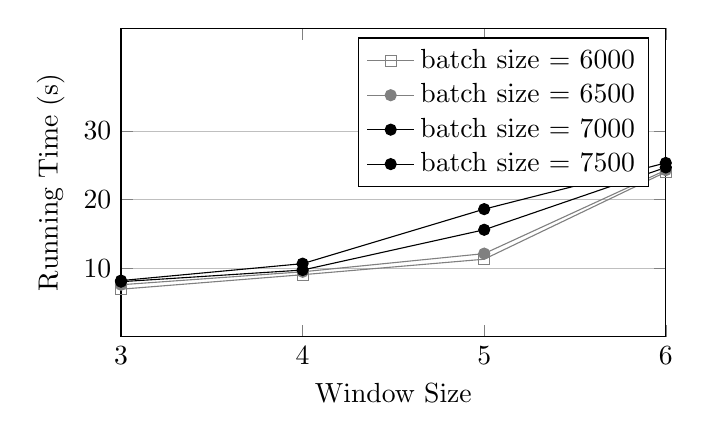
\begin{tikzpicture}
\begin{axis}[
    width=8.5cm,
    height=5.5cm,
    xlabel={Window Size},
    ylabel={Running Time (s)},
    xmin=3, xmax=6,
    ymin=0, ymax=45,
    xtick={3,4,5,6},
    ytick={10,20,30},
    legend pos=north east,
    ymajorgrids=true,
    grid style={line width=.2pt,draw=gray!50},
]
 
\addplot[
    solid,color=gray, every mark/.append style={solid, fill=gray}, mark=square
    ]
    coordinates {
		(3,6.935 )
		(4,9.048 )
		(5,11.308)
		(6,24.026)

	};
    \addlegendentry{batch size $=$ 6000}

	\addplot[
    solid,color=gray, every mark/.append style={solid, fill=gray}, mark=*
    ]
    coordinates {
		(3,7.587)
		(4,9.473)
		(5,12.126)
		(6,24.299)
};
    \addlegendentry{batch size $=$ 6500}
	

\addplot[
    solid,color=black, every mark/.append style={solid, fill=black}, mark=*
    ]
    coordinates {
		(3,8.030)
		(4,9.729)
		(5,15.602)
		(6,24.690)

};
    \addlegendentry{batch size $=$ 7000}
	
	
\addplot[
    solid,color=black, every mark/.append style={solid, fill=black}, mark=*
    ]
    coordinates {
		(3,8.192)
		(4,10.662)
		(5,18.613)
		(6,25.351)
};
    \addlegendentry{batch size $=$ 7500}
\end{axis}
\end{tikzpicture}
%\end{document}